\documentclass[11pt]{article}
% Shared preamble for the Svetoch papers.
% Each paper.tex \input's this file (compile from inside the paper's folder):
%     \documentclass[11pt]{article}
%     % Shared preamble for the Svetoch papers.
% Each paper.tex \input's this file (compile from inside the paper's folder):
%     \documentclass[11pt]{article}
%     % Shared preamble for the Svetoch papers.
% Each paper.tex \input's this file (compile from inside the paper's folder):
%     \documentclass[11pt]{article}
%     \input{../tex/preamble.tex}
% Figures live in ../figures/*.pdf  (graphicspath set below).
\usepackage[utf8]{inputenc}
\usepackage[T1]{fontenc}
\usepackage{lmodern}
\usepackage[a4paper,margin=1in]{geometry}
\usepackage{amsmath,amssymb}
\usepackage{graphicx}
\graphicspath{{../figures/}}
\usepackage{booktabs}
\usepackage{caption}
\captionsetup{font=small,labelfont=bf}
% --- Minimal, siunitx-free unit support (so papers compile on any TeX install) ---
\usepackage{textcomp}
\newcommand{\SI}[2]{#1\,#2}
\newcommand{\si}[1]{#1}
\newcommand{\hertz}{Hz}
\newcommand{\meter}{m}
\newcommand{\centi}{c}
\newcommand{\milli}{m}
\newcommand{\micro}{\textmu}
\newcommand{\second}{s}
\newcommand{\kelvin}{K}
% ---------------------------------------------------------------------------------
\usepackage[colorlinks=true,linkcolor=blue,citecolor=blue,urlcolor=blue]{hyperref}
\usepackage{xcolor}
\definecolor{accent}{HTML}{6366F1}

% Common author block (add affiliation/ORCID if available before publishing)
\newcommand{\svetochauthor}{Oleg Yuryevich Kirichenko \\[4pt]
  \normalsize Independent researcher \\[2pt]
  \normalsize \href{mailto:urevich55@gmail.com}{urevich55@gmail.com} \quad\textbullet\quad GitHub: \href{https://github.com/infosave2007}{@infosave2007}}

\newcommand{\svetochfooter}{%
  \vspace{1em}\noindent\rule{\linewidth}{0.4pt}\\[2pt]
  {\footnotesize Part of the \emph{Svetoch} series (defensive publication, not patented).
  Project and code: \href{https://github.com/infosave2007/svetoch}{github.com/infosave2007/svetoch};
  related VMF/NVG theory: \href{https://github.com/infosave2007/vmf}{github.com/infosave2007/vmf}.
  Released for the public record to establish authorship and priority.}}

% Figures live in ../figures/*.pdf  (graphicspath set below).
\usepackage[utf8]{inputenc}
\usepackage[T1]{fontenc}
\usepackage{lmodern}
\usepackage[a4paper,margin=1in]{geometry}
\usepackage{amsmath,amssymb}
\usepackage{graphicx}
\graphicspath{{../figures/}}
\usepackage{booktabs}
\usepackage{caption}
\captionsetup{font=small,labelfont=bf}
% --- Minimal, siunitx-free unit support (so papers compile on any TeX install) ---
\usepackage{textcomp}
\newcommand{\SI}[2]{#1\,#2}
\newcommand{\si}[1]{#1}
\newcommand{\hertz}{Hz}
\newcommand{\meter}{m}
\newcommand{\centi}{c}
\newcommand{\milli}{m}
\newcommand{\micro}{\textmu}
\newcommand{\second}{s}
\newcommand{\kelvin}{K}
% ---------------------------------------------------------------------------------
\usepackage[colorlinks=true,linkcolor=blue,citecolor=blue,urlcolor=blue]{hyperref}
\usepackage{xcolor}
\definecolor{accent}{HTML}{6366F1}

% Common author block (add affiliation/ORCID if available before publishing)
\newcommand{\svetochauthor}{Oleg Yuryevich Kirichenko \\[4pt]
  \normalsize Independent researcher \\[2pt]
  \normalsize \href{mailto:urevich55@gmail.com}{urevich55@gmail.com} \quad\textbullet\quad GitHub: \href{https://github.com/infosave2007}{@infosave2007}}

\newcommand{\svetochfooter}{%
  \vspace{1em}\noindent\rule{\linewidth}{0.4pt}\\[2pt]
  {\footnotesize Part of the \emph{Svetoch} series (defensive publication, not patented).
  Project and code: \href{https://github.com/infosave2007/svetoch}{github.com/infosave2007/svetoch};
  related VMF/NVG theory: \href{https://github.com/infosave2007/vmf}{github.com/infosave2007/vmf}.
  Released for the public record to establish authorship and priority.}}

% Figures live in ../figures/*.pdf  (graphicspath set below).
\usepackage[utf8]{inputenc}
\usepackage[T1]{fontenc}
\usepackage{lmodern}
\usepackage[a4paper,margin=1in]{geometry}
\usepackage{amsmath,amssymb}
\usepackage{graphicx}
\graphicspath{{../figures/}}
\usepackage{booktabs}
\usepackage{caption}
\captionsetup{font=small,labelfont=bf}
% --- Minimal, siunitx-free unit support (so papers compile on any TeX install) ---
\usepackage{textcomp}
\newcommand{\SI}[2]{#1\,#2}
\newcommand{\si}[1]{#1}
\newcommand{\hertz}{Hz}
\newcommand{\meter}{m}
\newcommand{\centi}{c}
\newcommand{\milli}{m}
\newcommand{\micro}{\textmu}
\newcommand{\second}{s}
\newcommand{\kelvin}{K}
% ---------------------------------------------------------------------------------
\usepackage[colorlinks=true,linkcolor=blue,citecolor=blue,urlcolor=blue]{hyperref}
\usepackage{xcolor}
\definecolor{accent}{HTML}{6366F1}

% Common author block (add affiliation/ORCID if available before publishing)
\newcommand{\svetochauthor}{Oleg Yuryevich Kirichenko \\[4pt]
  \normalsize Independent researcher \\[2pt]
  \normalsize \href{mailto:urevich55@gmail.com}{urevich55@gmail.com} \quad\textbullet\quad GitHub: \href{https://github.com/infosave2007}{@infosave2007}}

\newcommand{\svetochfooter}{%
  \vspace{1em}\noindent\rule{\linewidth}{0.4pt}\\[2pt]
  {\footnotesize Part of the \emph{Svetoch} series (defensive publication, not patented).
  Project and code: \href{https://github.com/infosave2007/svetoch}{github.com/infosave2007/svetoch};
  related VMF/NVG theory: \href{https://github.com/infosave2007/vmf}{github.com/infosave2007/vmf}.
  Released for the public record to establish authorship and priority.}}


\title{\textbf{Hardware Neural-Network Primitives from\\ Commodity Display Physics}\\[4pt]
{\large Svetoch Series, Paper II of VI}}
\author{\svetochauthor}
\date{17 June 2026}

\begin{document}
\maketitle

\begin{abstract}
\noindent Paper~I showed that an unmodified smartphone plus an inexpensive mirror evaluates a
multiply--accumulate in light. Here we make a complementary observation: the \emph{same}
commodity display and sensor hardware that carries the operands also supplies, for free,
several of the non-linear and stateful operators a neural network needs around its matrix
multiplications. We identify and characterise four such \textbf{hardware primitives} on a
Xiaomi 12 Lite. (1)~The OLED's monotonic electro-optical $\gamma$-characteristic acts as a
hardware activation (SiLU/Swish/ReLU-like); we quantify it as the deviation of the measured
code-to-light transfer from a straight line, $1-R^2_\text{lin}$, on the curve Paper~I fit to
$\gamma=1.10$, $R^2=0.96$ (SNR $8.2$ bits). (2)~Finite OLED pixel response time stores a
fading trace of the previous frame, isomorphic to an LSTM forget gate
$\alpha=\exp(-\Delta t/\tau)$ --- a recurrence whose gate is set by \emph{physics}, not by
training. (3)~Displaying Key and Value patterns in different colour channels lets the camera's
Bayer mosaic separate two attention ``heads'' in one exposure. (4)~Lens chromatic aberration
focuses R/G/B differently, marking token position by spatial frequency and colour --- a
positional encoding with no arithmetic. We report each primitive honestly: the
$\gamma$-activation and persistence-memory effects are robust and measured; Bayer multiplexing
rests on known physics whose novelty is only in the framing; the chromatic positional signal
is weak and its cross-device reproducibility is an open question.
\end{abstract}

\noindent\textbf{Keywords:} hardware activation function, OLED gamma curve, in-sensor
computing, recurrent memory, LSTM, Bayer filter, attention, chromatic aberration, positional
encoding, optical neural networks, edge AI.

\section{Introduction}
A neural network is not only matrix multiplications. Between its linear layers sit pointwise
non-linearities (activations), and around them sit stateful and structural operators ---
recurrence, attention, positional encoding. Paper~I demonstrated that the heavy linear algebra
can be offloaded to an OLED--mirror--camera optical channel. The natural next question is
whether the \emph{non-linear and structural} operators must then return to the CPU, or whether
the same display-and-sensor physics already implements them.

We argue that it does, and that this is not a coincidence: an emissive display and an
integrating image sensor are rich analog devices whose ``imperfections'' --- a non-linear
transfer curve, finite pixel decay, a colour mosaic, a dispersive lens --- map cleanly onto
operators that practitioners otherwise compute explicitly. Treating these as \emph{features}
rather than \emph{defects} yields neural-network primitives that consume no CPU arithmetic.
This paper characterises four such primitives on the reference device (Section~\ref{sec:prim}),
shows how they compose into a hybrid coprocessor (Section~\ref{sec:compose}), gives the
protocol (Section~\ref{sec:methods}), and is deliberately careful about which claims are strong
and which are plausible-but-weak (Section~\ref{sec:disc}).

\section{The four primitives}
\label{sec:prim}

\subsection{Gamma-curve activation}
The map from digital drive level $u\in[0,1]$ to emitted (and captured) light $y$ is not
linear: an OLED applies a monotonic electro-optical $\gamma$-curve, well approximated by a
power law
\begin{equation}
y = u^{\gamma}, \qquad \gamma = 1.10 \;\; (R^2 = 0.96),
\end{equation}
measured on the reference channel (Figure~\ref{fig:gamma}, the curve calibrated in Paper~I).
If a number is encoded as pixel brightness, then displaying it and reading it back applies this
monotone non-linearity automatically --- exactly the role of an activation after a linear
layer. The smooth, monotone, slightly super-linear shape is qualitatively SiLU/Swish-like (and
clips toward a ReLU-like floor at black); the designer chooses the encoding so the operating
point lands on the useful part of the curve. We quantify the \emph{degree} of activation as the
deviation of the transfer curve from a straight line,
\begin{equation}
\mathcal{N} = 1 - R^2_\text{lin},
\end{equation}
where $R^2_\text{lin}$ is the coefficient of determination of a \emph{linear} fit to the same
$(u,y)$ data: $\mathcal{N}=0$ is a linear channel (no activation), $\mathcal{N}\to 1$ a
strongly non-linear one. The contribution is that a free, calibrated, monotone non-linearity
exists at all, requiring zero CPU operations, and that its strength is one measured number per
device.

\begin{figure}[ht]\centering
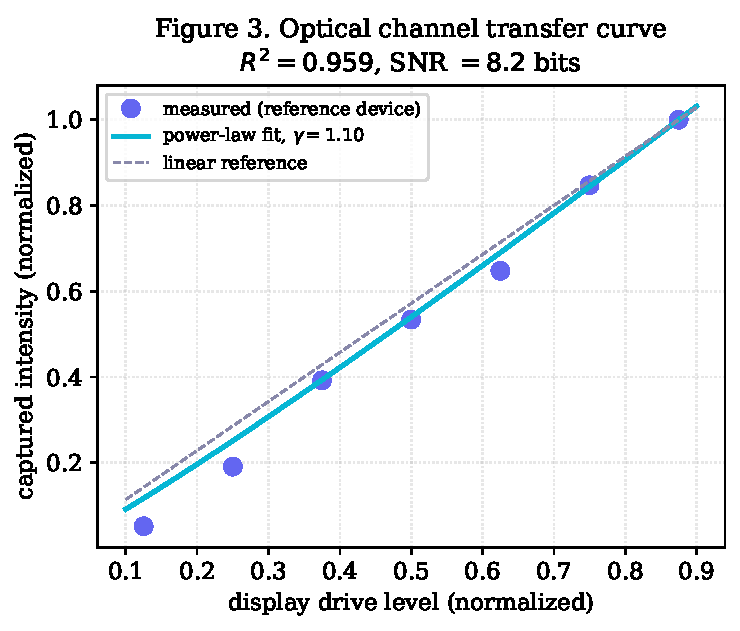
\includegraphics[width=0.56\linewidth]{fig03_gamma_curve.pdf}
\caption{Measured optical-channel transfer curve (reference device): captured intensity vs.
drive level; power-law fit ($\gamma=1.10$, $R^2=0.96$); linear reference. The gap between the
two curves is the hardware non-linearity $\mathcal{N}=1-R^2_\text{lin}$ available as a free
activation.}
\label{fig:gamma}
\end{figure}

\subsection{OLED-persistence recurrent memory}
A network that processes a sequence needs state. The reference primitive is the LSTM forget
gate, which retains a fraction of the previous cell state each step. An OLED pixel already does
this physically: its luminance does not switch instantaneously but decays with a finite
afterglow time constant $\tau$ (order $1$--$5$\,ms for the emissive layer). When frames are
presented at interval $\Delta t$, frame $n$ is read on top of a fading residual of frame
$n-1$:
\begin{equation}
y_n = x_n + \alpha\, y_{n-1}, \qquad \alpha = \exp\!\left(-\frac{\Delta t}{\tau}\right),
\end{equation}
a first-order recurrence --- a leaky integrator, the linearised core of an LSTM/GRU memory
cell. The decisive point is that \textbf{the forget gate $\alpha$ is set by device physics, not
learned}: it is fixed by $\tau$ and chosen operationally by $\Delta t$. Figure~\ref{fig:lstm}
shows the residual frame-to-frame correlation decaying as $\exp(-\Delta t/\tau)$ for
$\Delta t = 30, 60, 120$\,ms, i.e.\ the measured forget-gate curve.

\begin{figure}[ht]\centering
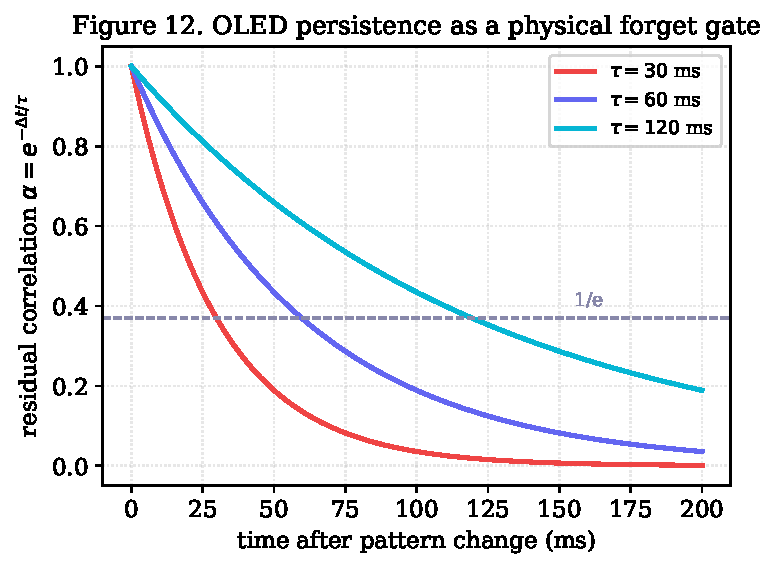
\includegraphics[width=0.58\linewidth]{fig12_lstm_decay.pdf}
\caption{OLED persistence as an LSTM forget gate. Residual frame-to-frame correlation
$\alpha=\exp(-\Delta t/\tau)$ vs.\ frame interval, for $\Delta t = 30/60/120$\,ms. The decay
constant $\tau$ --- a fixed device property --- sets the recurrence's memory horizon with no
trained parameters.}
\label{fig:lstm}
\end{figure}

\subsection{Bayer attention multiplexing}
Attention computes, per head, products of Query/Key/Value projections. We fold two such
products into one exposure using the camera's colour mosaic. Display the Key pattern in red and
the Value pattern in green \emph{simultaneously}; the CMOS Bayer colour-filter array
hardware-separates them on capture. Demosaicing yields two independent results from one frame
$I$:
\begin{equation}
\mathbf{r} = \mathcal{D}_R(I)\;\propto\;\text{(head 1)}, \qquad
\mathbf{g} = \mathcal{D}_G(I)\;\propto\;\text{(head 2)},
\end{equation}
so two attention heads are read in parallel at no extra optical or CPU cost --- a colour-space
analogue of multi-head attention. We are explicit about novelty: \textbf{Bayer colour
separation is itself entirely standard} sensor physics. The only non-obvious element is the
\emph{framing} --- assigning colour channels to distinct heads so one exposure yields two head
outputs. We present this as a useful engineering primitive, not a fundamental discovery.
Cross-talk (imperfect R/G isolation) bounds the head count; two (R, G) are robust, a third (B)
marginal.

\subsection{Chromatic positional encoding (Chromatic RoPE)}
Transformers need to know \emph{where} each token sits; rotary positional encoding (RoPE)
rotates feature pairs at position-dependent frequencies. A lens supplies a
position-and-colour-dependent signal for free via \textbf{chromatic aberration}: different
wavelengths focus at different planes, so each colour channel has a different
modulation-transfer function (MTF). Modelling the per-channel optics as
\begin{equation}
\text{MTF}_c(f) = \exp\!\left[-\left(\frac{f}{f_{0,c}}\right)^2\right], \qquad c\in\{R,G,B\},
\end{equation}
each colour $c$ has its own cutoff $f_{0,c}$ set by where that wavelength focuses; the contrast
a spatial frequency $f$ retains then depends jointly on $(f,c)$, tagging a token by spatial
frequency and colour with \textbf{no CPU arithmetic}. This is the weakest of the four
primitives, and we say so plainly: on the reference geometry the chromatic differential is
small (well-corrected lens, short path), close to the noise. The idea is clever and narrow,
but \textbf{its effect is weak and its cross-device reproducibility is the open question}. We
include it as a \emph{plausible} hardware positional-encoding mechanism warranting dedicated
validation, not as a demonstrated one.

\section{Composing them into a hybrid coprocessor}
\label{sec:compose}
Individually each primitive removes a small piece of CPU work; together they outline a hybrid
optical LLM coprocessor (Figure~\ref{fig:pipe}) in which \textbf{the CPU runs only control
logic}:
\begin{description}
\item[Linear algebra] ($\mathbf{W}_Q,\mathbf{W}_K,\mathbf{W}_V$, MLP) --- the
camera-integration MAC of Paper~I.
\item[Activation] --- the $\gamma$-curve, applied automatically by the encode-as-brightness
step between layers.
\item[Recurrence] --- OLED persistence, gate fixed by $\tau$, tuned by frame rate.
\item[Multi-head read-out] --- the Bayer colour split, two heads per exposure.
\item[Positional encoding] --- the chromatic-aberration signal (plausible, pending validation).
\end{description}
The processor's job collapses to sequencing frames, choosing encodings, and taking the final
$\arg\max$. This is the umbrella architecture: its strength equals the strength of its
components, so the strong primitives ($\gamma$-activation, persistence memory) carry it, while
the weaker ones (Bayer framing, chromatic encoding) are optional accelerators rather than
load-bearing claims.

\begin{figure}[ht]\centering
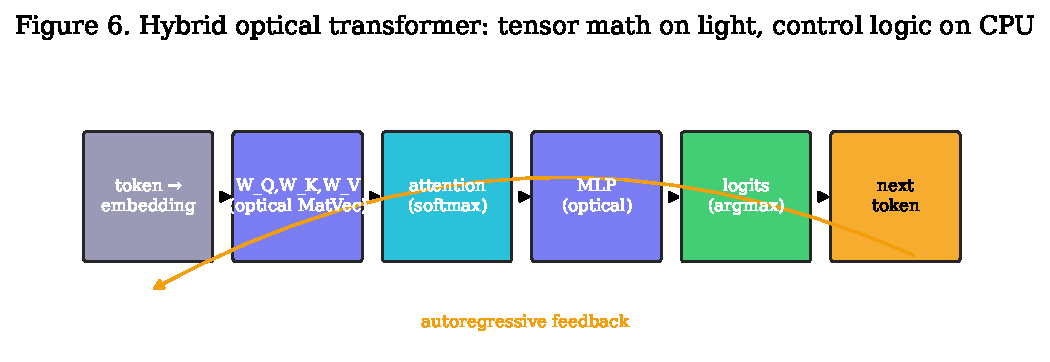
\includegraphics[width=0.92\linewidth]{fig06_pipeline.pdf}
\caption{Hybrid optical transformer pipeline. Heavy tensor arithmetic, the $\gamma$ activation,
the persistence recurrence, and the colour-split attention read-out all live in the
display/sensor physics; only control logic and the final $\arg\max$ run on the CPU. Dashed:
autoregressive feedback.}
\label{fig:pipe}
\end{figure}

\section{Methods}
\label{sec:methods}
\textbf{Hardware:} Xiaomi 12 Lite (6.55" AMOLED, $2400\times1080$, \SI{120}{\hertz}, pitch
\SI{63.2}{\micro\meter}; 32\,MP front camera, min.\ focus $\approx$\SI{10}{\centi\meter}). For
primitives needing the reflected channel (activation read-back, attention multiplexing) the
phone lies screen-down over a flat mirror at gap $d\approx 3$--$5$\,cm, as in Paper~I; the
persistence and chromatic primitives are largely device-intrinsic.
\textbf{$\gamma$-activation:} sweep $u$ over a calibrated ramp, capture white-normalised $y$,
fit a power law ($\gamma$, $R^2$) and a line ($R^2_\text{lin}$), report
$\mathcal{N}=1-R^2_\text{lin}$. \textbf{Persistence:} display an impulse then black frames at
fixed $\Delta t$; measure residual correlation; fit $\alpha=\exp(-\Delta t/\tau)$ for
$\Delta t = 30, 60, 120$\,ms. \textbf{Bayer multiplexing:} display distinct R and G patterns in
one frame; demosaic; read R/G planes as two products; report channel cross-talk.
\textbf{Chromatic:} display gratings of several spatial frequencies per colour; measure
per-channel Michelson contrast; report per-colour cutoff differences and run-to-run scatter.
\textbf{Software:} as in Paper~I, a dependency-free Python HTTPS server and browser ES-module
stages; figures by \texttt{papers/scripts/make\_figures.py} (real-data figures use the
reference run 2026-06-06; model figures are labelled).

\section{Discussion \& limitations}
\label{sec:disc}
The unifying claim is modest and, we think, durable: \textbf{the analog physics of a commodity
display and sensor already implements neural-network operators otherwise computed in software},
and at least two --- the $\gamma$-curve activation and the persistence recurrence --- are
robust, measured, and free of CPU arithmetic. The activation has no obvious prior art in the
``display $\gamma$ as activation'' framing; the persistence-as-forget-gate recurrence is, to
our knowledge, novel and honestly grounded in a measured time constant.

We are equally clear about the limits. (i)~\emph{Strength of non-linearity:} on a well-behaved
panel $\gamma$ is near unity, so the activation is gentle; deeper non-linearity needs operating
near clipping or stacking the channel, both costing SNR. (ii)~\emph{Bayer multiplexing is a
framing, not a discovery:} colour-channel separation is textbook physics; only the ``parallel
attention heads'' interpretation is new, and cross-talk limits it to roughly two clean heads.
(iii)~\emph{Chromatic encoding is weak:} the per-channel MTF differential is small and close to
noise, and cross-phone reproducibility is unresolved --- a hypothesis, not a result.
(iv)~\emph{Device specificity:} $\gamma$, $\tau$, Bayer cross-talk, and chromatic cutoffs are
per-device constants requiring re-measurement on new hardware; cross-device scaling is the
principal open validation. (v)~These primitives accelerate but do not by themselves make a fast
accelerator --- the channel throughput of Paper~I remains the binding constraint.

\section{Conclusion}
Around the optical matrix engine of Paper~I, the same smartphone supplies several
neural-network operators for free: a $\gamma$-curve activation of strength
$\mathcal{N}=1-R^2_\text{lin}$; a recurrent forget gate $\alpha=\exp(-\Delta t/\tau)$ fixed by
physics; a Bayer mosaic separating two attention heads per exposure; and chromatic aberration
that may mark token position. The first two are demonstrated and strong; the last two are
plausible primitives reported with their caveats. Composed, they sketch a hybrid optical
coprocessor in which the CPU does only control logic.

\paragraph{Data and code.} \href{https://github.com/infosave2007/svetoch}{github.com/infosave2007/svetoch}; related VMF/NVG theory: \href{https://github.com/infosave2007/vmf}{github.com/infosave2007/vmf}
(Apache-2.0).
\paragraph{Priority note.} Released as a defensive publication to establish authorship and date
of disclosure; the author has elected not to seek patent protection.

\begin{thebibliography}{9}\small
\bibitem{swish} P. Ramachandran, B. Zoph, Q. V. Le, ``Searching for activation functions,'' \emph{arXiv:1710.05941} (2017).
\bibitem{lstm} S. Hochreiter, J. Schmidhuber, ``Long short-term memory,'' \emph{Neural Computation} \textbf{9}, 1735 (1997).
\bibitem{rope} J. Su et al., ``RoFormer: Enhanced transformer with rotary position embedding,'' \emph{arXiv:2104.09864} (2021).
\bibitem{bayer} B. E. Bayer, ``Color imaging array,'' U.S. Patent 3,971,065 (1976).
\bibitem{wetzstein} G. Wetzstein et al., ``Inference in AI with deep optics and photonics,'' \emph{Nature} \textbf{588}, 39 (2020).
\end{thebibliography}

\svetochfooter
\end{document}
